\section{Missions}
\label{missions}
Le moyen de présenter les concepts retenus pour dans Rsnap est une approche par mission. Cette solution a été retenue par l'analyse des autres initiatives similaires dans le chapitre \ref{travail associé}. Dans le cadre de ce travail, une série de missions ont été produite pour avoir une plateforme utilisable.\\

Une fois le choix de l'approche par mission choisit, nous avons défini comment nous allions amener la théorie de la programmation à travers ces missions. Il s'est avéré pour capter l'attention et l'intérêt des étudiants, il était nécessaire d'introduire les missions par la présentation d'un but final. Celui retenu dans ce travail a été le jeu du chien et du chat. Dans ce jeu le chien doit courir après le chat et le manger. Le principe de ce jeu est très simple et permet l'introduction de plusieurs concepts de programmation intéressants tels que la condition, les boucles et également les événements.\\

Pour introduire les concepts de manière douce, la mission finale est introduite par trois missions d'introduction : \texttt{la voiture}, \texttt{l'hélicoptère} et \texttt{Soyons courtois}. Dans la suite de cette partie, nous allons décrire les missions et faire une analyse des concepts introduits.

\subsection{Voiture}
\label{mission-voiture}
Dans cette première mission, voir figure \ref{fig:mission-voiture}, les participants étaient mis dans un bolide qui devait atteindre la ligne d'arrivée en restant sur la route. Si la voiture sortait de la route, elle explosait, à chaque lancement du scripte la voiture reprenait sa position d'origine.

Cette mission avait pour but que les participants puissent prendre en main l'interface de Snap! BYOB et d'introduire la notion de suite d'instruction. En effet, le fait de devoir prévoir les instructions n'est pas un concept facile pour le public cible. Beaucoup exécutent une opération et puis cherche à savoir comment continuer à partir de leur nouvelle position. Ici la voiture retournant chaque fois à sont point de départ, nous forcions les participants a réfléchir de manière globale et non une action à l'avance.

\begin{figure}[ht]
  \begin{center}
    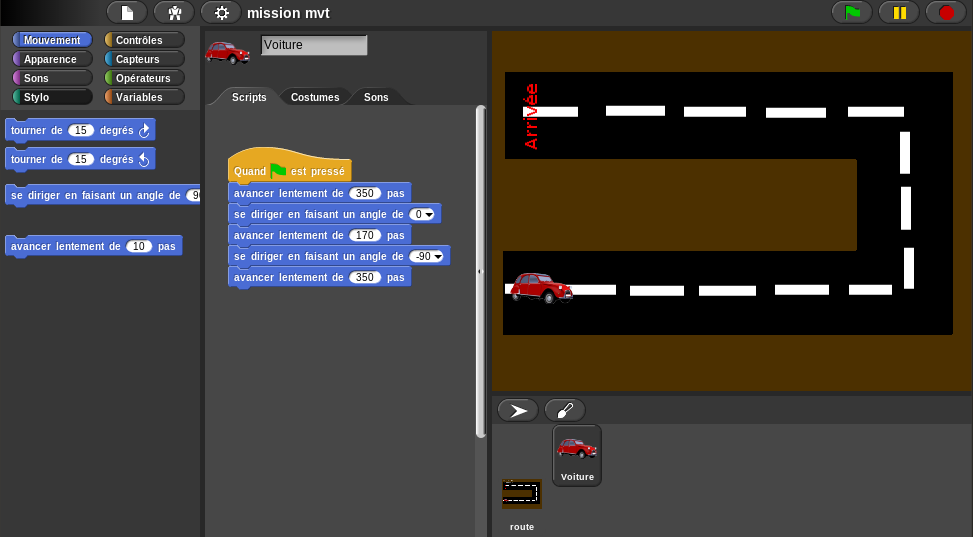
\includegraphics[scale=0.35]{content/7-solution/1-missions/images/voiture}
    \caption{Mission de la voiture}
    \label{fig:mission-voiture}
  \end{center}
\end{figure}


\subsection{L'hélicoptère}
\label{mission-helicoptere}
Pour cette mission, voir figure \ref{fig:mission-hélicoptère}, les participants étaient aux commandes d'un hélicoptère. Leur but est de faire le tour de la piste. La piste est un ellipsoïde border d'herbe. Si l'hélicoptère touche l'herbe, il explose et comme pour le précédent, à chaque lancement de scripte l'hélicoptère se repositionnait à son point de départ. Ceci toujours dans le but de forcer les participants à voir la solution dans son ensemble et non juste a la prochaine étape. En plus, l'herbe et de la piste, sur le contour extérieur de la piste est positionner une bande rouge et à l'intérieur elle est bleu. Le but est de tournée des qu'une de ces deux couleurs est touchée et ce pour évité l'herbe.\\

Les concepts introduits par cette mission sont :
\begin{itemize}
\item les boucles, particulièrement le \texttt{while} ;
\item la gestion des collisions grâce au capteur de couleur ;
\item la division en sous process (un pour avancer, un pour la collision rouge et un pour la bleu).
\end{itemize}
\begin{figure}[ht]
  \begin{center}
    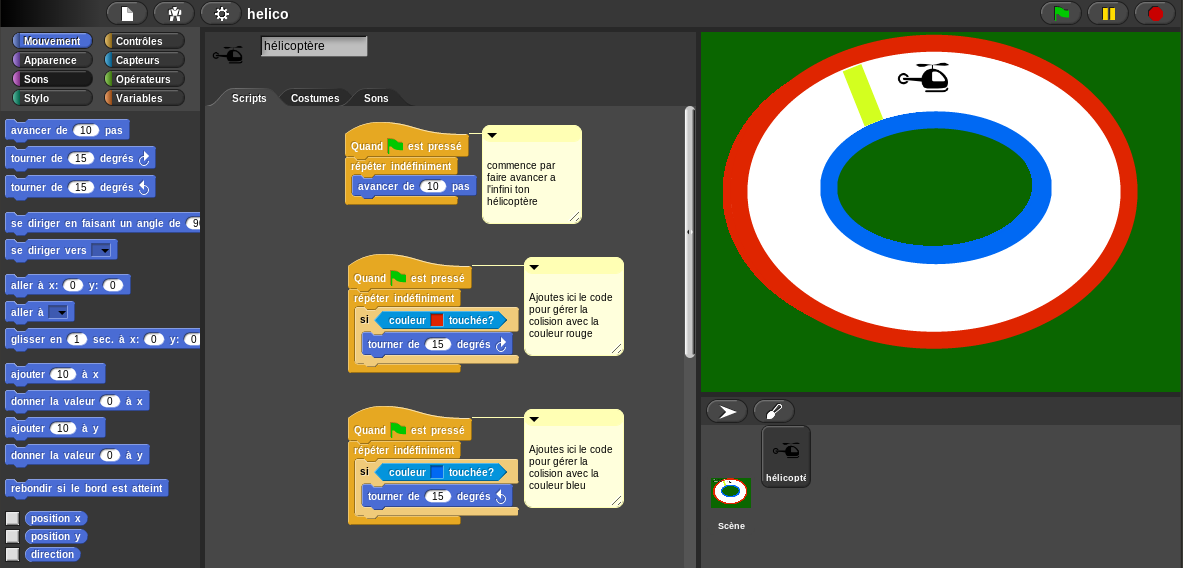
\includegraphics[scale=0.3]{content/7-solution/1-missions/images/helicoptere}
    \caption{Mission de l'hélicoptère}
    \label{fig:mission-hélicoptère}
  \end{center}
\end{figure}

\subsection{Soyons courtois}
\label{mission-courtois}
Dans cette dernière mission de préparation, voir figure \ref{fig:courtois}, les participants se retrouvent à diriger un personnage qui croise d'autres personnages. Ces derniers disent bonjour à chaque qu'ils croisent quelqu'un. Le but de la mission est dire bonjour également quand le personnage du participant croise quelqu'un.

Les concepts introduits par cette mission sont :
\begin{itemize}
\item la gestion des collisions grâce au capteur de sprite ;
\item la division en sous process (un pour chaque personne) ;
\item Introduction à l'interactivité de l'interface (faire déplacer un personnage) ;
\item la gestion des dialogues et affichage de texte.
\end{itemize}
\begin{figure}[ht]
  \begin{center}
    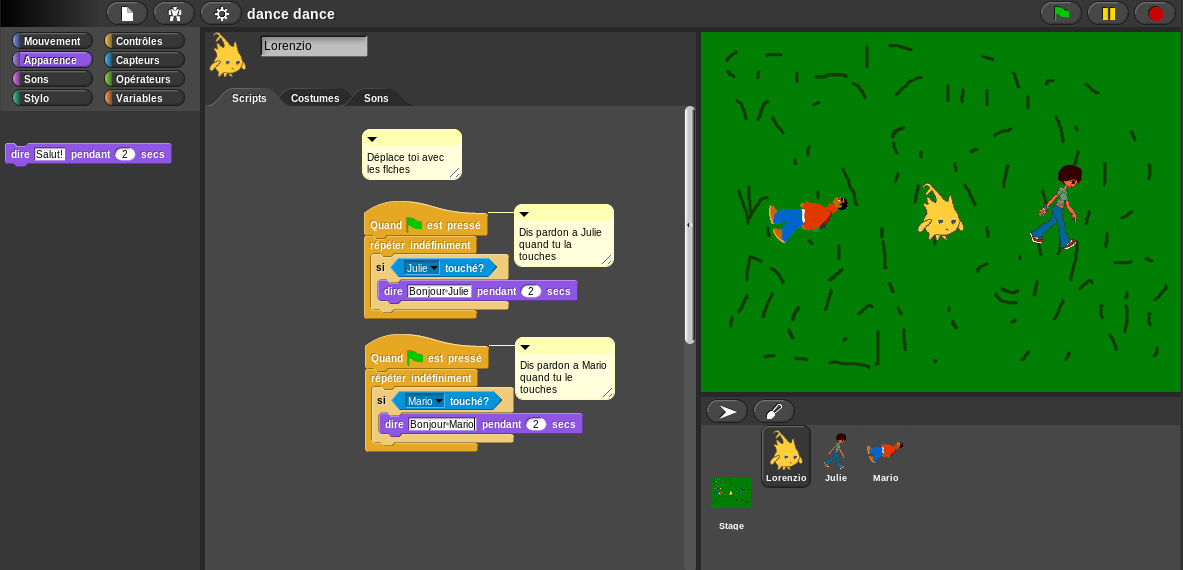
\includegraphics[scale=0.3]{content/7-solution/1-missions/images/courtois}
    \caption{Mission de soyons courtois}
    \label{fig:courtois}
  \end{center}
\end{figure}
\subsection{Chien et chat}
\label{chien-chat}
Cette mission est la dernière de la série et a pour but de mettre ensemble tous les concepts vus dans les missions de préparations. Dans cette mission, les étudiants doivent faire en sorte d'avoir deux personnages et de pouvoir les déplacer séparément à l'aide des touches. Le chien doit courir après le chat. Si celui-ci est touché par le chien il crie et le chien gagne un point.\\

Cette mission reprend les concepts vus dans les missions de préparation au quels il faut ajouter:
\begin{itemize}
\item la gestion des variables à travers la variable de score ;
\item l'activation d'un script sur un événement pour les déplacements ;
\end{itemize}

Pour les déplacements, il est déjà présent dans la mission précédente, mais à l'état passif. Ils ne font que l'utiliser, ils ne l'ont pas crée eux-mêmes. Dans cette mission, ils doivent le faire tout seuls. Ceci permet de bien fixer ce concept qui est important dès qu'une interaction clavier est souhaitée.

%analyse mission voiture, cela à permis de prendre en main les entrées des blocs. Au début, beaucoup prennent 3 blocs avancer de 10 pas pour faire 30 pas au lieu de changer la valeur du 10 en 30.
